Checkers also known as draughts is a ancient board game. A simplified
version can be described as follows:
\begin{quote}
  Checkers is a turn-based strategy game for two players. The game is
  (typically) played on an $8\times8$ checkerboard of alternating
  dark- and light-colored squares. Each player starts with 12 pieces, where
  player one's pieces are light, and player two's pieces are dark in
  color, and the initial position of the pieces is shown in
  Figure~\ref{fig:checkers}.
  \begin{figure}
    \centering
    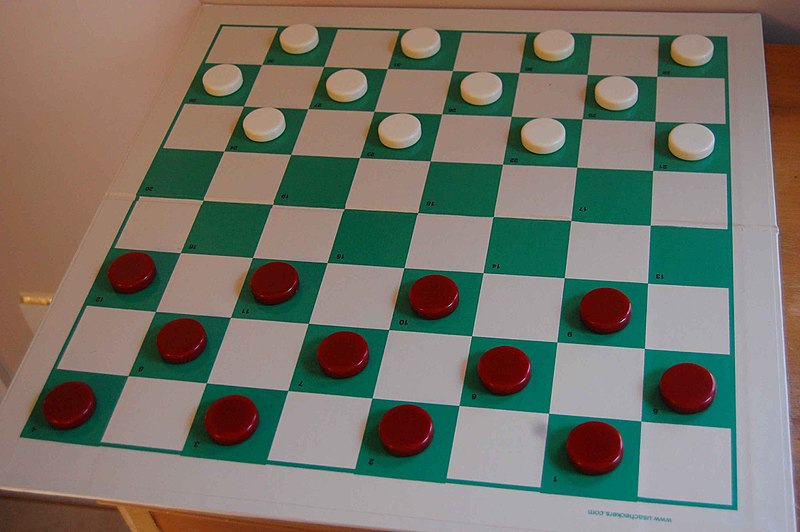
\includegraphics[width=0.3\textwidth]{800px-CheckersStandard}
    \caption{The starting position in Checkers [\url{https://commons.wikimedia.org/wiki/File:CheckersStandard.jpg}]}
    \label{fig:checkers}
  \end{figure}
  Players take turns moving one of their pieces. A player must move a
  piece if possible, and when one player has no more pieces, then that
  player has lost the game.

  A piece may only move diagonally into an unoccupied adjacent
  square. If the adjacent square contains an opponent's piece and the
  square immediately beyond is vacant, then the piece jumps over the
  opponent's piece and the opponent's piece is removed from the
  board.
\end{quote}
Use the nouns-and-verbs method to identify possible classes and their
interactions and write 1-2 lines of description for each.